\documentclass[xcolor=table]{beamer}
%------------------------------------------------------------
% Theme and Appearance
%------------------------------------------------------------
\usetheme[footline=authorinstitutetitle]{Berlin} 
\setbeamertemplate{navigation symbols}{} 

% Headline with Access Code
\setbeamertemplate{headline}{
    \begin{beamercolorbox}[wd=\paperwidth,ht=2.5ex,dp=1ex,right]{section in head/foot}
        \usebeamerfont{section in head/foot}
        \hspace{0.5cm}
        \ifnum\insertframenumber<30
            \raisebox{-1pt}[0pt][0pt]{\normalsize\textbf{Attendance Code: 871550}}
        \fi
        \hspace{0.5cm}
    \end{beamercolorbox}
}
% Footline with page numbers
\setbeamertemplate{footline}{
    \leavevmode%
    \hbox{%
        \begin{beamercolorbox}[wd=.333333\paperwidth,ht=2.25ex,dp=1ex,left]{author in head/foot}%
            \usebeamerfont{author in head/foot}\hspace*{0.5em}\insertshortauthor
        \end{beamercolorbox}%
        \begin{beamercolorbox}[wd=.333333\paperwidth,ht=2.25ex,dp=1ex,center]{title in head/foot}%
            \usebeamerfont{title in head/foot}\insertshorttitle
        \end{beamercolorbox}%
        \begin{beamercolorbox}[wd=.333333\paperwidth,ht=2.25ex,dp=1ex,right]{date in head/foot}%
            \usebeamerfont{date in head/foot}\insertshortdate{}\hspace*{2em}
            \insertframenumber{} / \inserttotalframenumber\hspace*{2ex} 
        \end{beamercolorbox}}%
    \vskip0pt%
}
\usepackage[utf8]{inputenc}
\usepackage[table]{xcolor}
\usepackage{colortbl}
\usepackage{minted}
\usepackage{lmodern}
\usepackage{tgheros}
\usepackage{hyperref}
\usepackage{tikz}
\usetikzlibrary{shapes, arrows, positioning, shadows, fit, calc, shapes.multipart, shapes.geometric, arrows.meta}

\renewcommand*\familydefault{\sfdefault}

% Agenda at the start of every section
\AtBeginSection[]
{
    \begin{frame}
        \frametitle{Agenda}
        \tableofcontents[currentsection]
    \end{frame}
}

%------------------------------------------------------------
% Title Page Information
%------------------------------------------------------------
\title[CMP9134 - Week 4]{Software System Modelling \& UML}
\subtitle{CMP9134: Software Engineering}
\author[Francesco Del Duchetto]{Dr Francesco Del Duchetto\\Lecturer in Robotics and Autonomous Systems}
\institute[University of Lincoln]{University of Lincoln}
\date{27 February 2026}

%------------------------------------------------------------
\begin{document}

%--- TITLE FRAME ---
\begin{frame}
    \titlepage
\end{frame}

%--- AGENDA FRAME ---
\begin{frame}
    \frametitle{Today's Agenda}
    \tableofcontents
\end{frame}

%------------------------------------------------------------
\section{Recap: Week 3}
%------------------------------------------------------------

\begin{frame}
    \frametitle{Recap: Requirements \& LEPSI}
    Last week, we moved from abstract planning to defining strict system boundaries and constraints.
    
    \begin{itemize}
        \item \textbf{Requirements Engineering:} Bridging the gap between what the customer wants and what the developers build.
        \item \textbf{Functional vs. Non-Functional:} What the system \textit{does} vs. \textit{how well} (or how securely) it does it.
        \item \textbf{LEPSI as Constraints:} We learned that Legal (GDPR), Ethical (Dual-Use), Professional, and Social (WCAG) issues act as strict Non-Functional Requirements.
        \item \textbf{Agile Implementation:} Translating requirements into User Stories with a strict \textbf{Definition of Done (DoD)}.
    \end{itemize}
\end{frame}

\begin{frame}
    \frametitle{Today's Learning Objectives}
    By the end of this lecture, you should be able to:
    \begin{enumerate}
        \item \textbf{Explain} the purpose of software system modelling and the concept of abstraction.
        \item \textbf{Identify} the standard UML (Unified Modeling Language) diagram types and their distinct perspectives.
        \item \textbf{Map} Object-Oriented Programming (OOP) concepts directly to UML Class Diagrams.
        \item \textbf{Select and apply} the appropriate models to visually represent a software system architecture.
    \end{enumerate}
\end{frame}

%------------------------------------------------------------
\section{Introduction to System Modelling}
%------------------------------------------------------------

\begin{frame}
    \frametitle{What is System Modelling?}
    \begin{block}{Definition}
        System modelling is the process of developing abstract models of a system, with each model presenting a different view or perspective of that system.
    \end{block}
    
    \vspace{0.3cm}
    \textbf{Why do we model?}
    \begin{itemize}
        \item To help the analyst understand the functionality of the system.
        \item To communicate with customers (who may not understand code).
        \item To provide a blueprint for developers before coding begins.
        \item To serve as documentation for future maintenance and updates.
    \end{itemize}
\end{frame}

\begin{frame}
    \frametitle{System Perspectives}
    A single model cannot capture everything. We use different models to represent different \textbf{perspectives}:
    
    \vspace{0.3cm}
    \begin{itemize}
        \item \textbf{External perspective:} Models the context or environment of the system.
        \item \textbf{Interaction perspective:} Models the interactions between a system and its environment, or between its components.
        \item \textbf{Structural perspective:} Models the organization of a system or the structure of the data that is processed.
        \item \textbf{Behavioral perspective:} Models the dynamic behavior of the system and how it responds to events.
    \end{itemize}
\end{frame}


\begin{frame}[fragile]
    \frametitle{The Power of a Software Model}
    \small
    \begin{block}{Abstraction in Action}
        A good model strips away the code to immediately communicate \textbf{how the system works} and its logical flow to anyone in the room.
    \end{block}
    
    \vspace{0.2cm}
    \textbf{Example: you can probably guess what is being modelled here...}
    
    \vspace{0.2cm}
    \centering
    \resizebox{0.95\textwidth}{!}{
    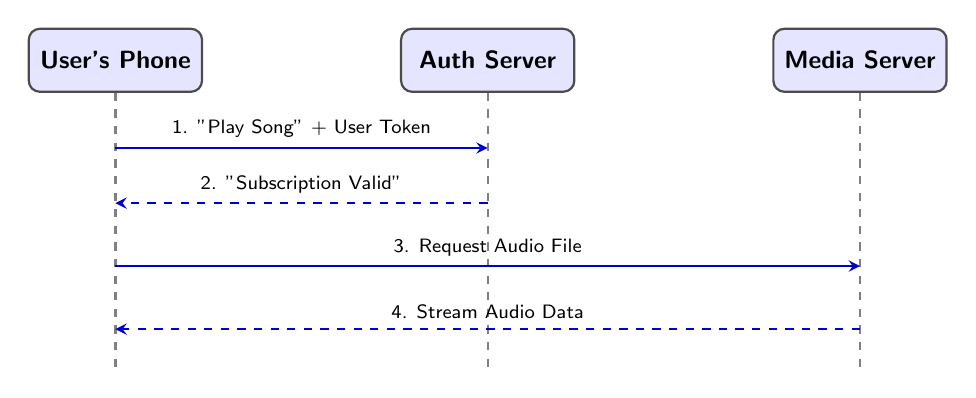
\begin{tikzpicture}[
        node distance=2.5cm,
        actor/.style={rectangle, draw=black!70, fill=blue!10, thick, minimum width=2.2cm, minimum height=0.8cm, rounded corners, font=\small\bfseries},
        arrow/.style={->, >=stealth, thick, blue!80!black}
    ]
        % Nodes
        \node[actor] (user) {User's Phone};
        \node[actor, right=2.5cm of user] (auth) {Auth Server};
        \node[actor, right=2.5cm of auth] (media) {Media Server};

        % Lifelines
        \draw[dashed, thick, gray] (user.south) -- +(0, -3.5);
        \draw[dashed, thick, gray] (auth.south) -- +(0, -3.5);
        \draw[dashed, thick, gray] (media.south) -- +(0, -3.5);

        % Messages
        \draw[arrow] ([yshift=-0.7cm]user.south) -- ([yshift=-0.7cm]auth.south) node[midway, above, font=\scriptsize, text=black] {1. "Play Song" + User Token};
        \draw[arrow, dashed] ([yshift=-1.4cm]auth.south) -- ([yshift=-1.4cm]user.south) node[midway, above, font=\scriptsize, text=black] {2. "Subscription Valid"};
        \draw[arrow] ([yshift=-2.2cm]user.south) -- ([yshift=-2.2cm]media.south) node[midway, above, font=\scriptsize, text=black] {3. Request Audio File};
        \draw[arrow, dashed] ([yshift=-3.0cm]media.south) -- ([yshift=-3.0cm]user.south) node[midway, above, font=\scriptsize, text=black] {4. Stream Audio Data};
    \end{tikzpicture}
    }
    
    % \vspace{0.4cm}
    \raggedright
    \footnotesize
    \begin{itemize}
        \item You instantly understand the \textbf{architecture} (Phone, Auth, Media).
        \item You understand the \textbf{logic} (You cannot stream audio without verifying the subscription first).
        \item You completely understand the feature \textbf{without needing to know if it is written in Python, Java, or C++!}
    \end{itemize}
\end{frame}


%------------------------------------------------------------
\section{UML Overview \& Key Diagrams}
%------------------------------------------------------------

\begin{frame}
    \frametitle{The Unified Modeling Language (UML)}
    UML is the industry standard for visualizing, specifying, constructing, and documenting the artifacts of a software-intensive system.
    
    % insert image
    \begin{center}
        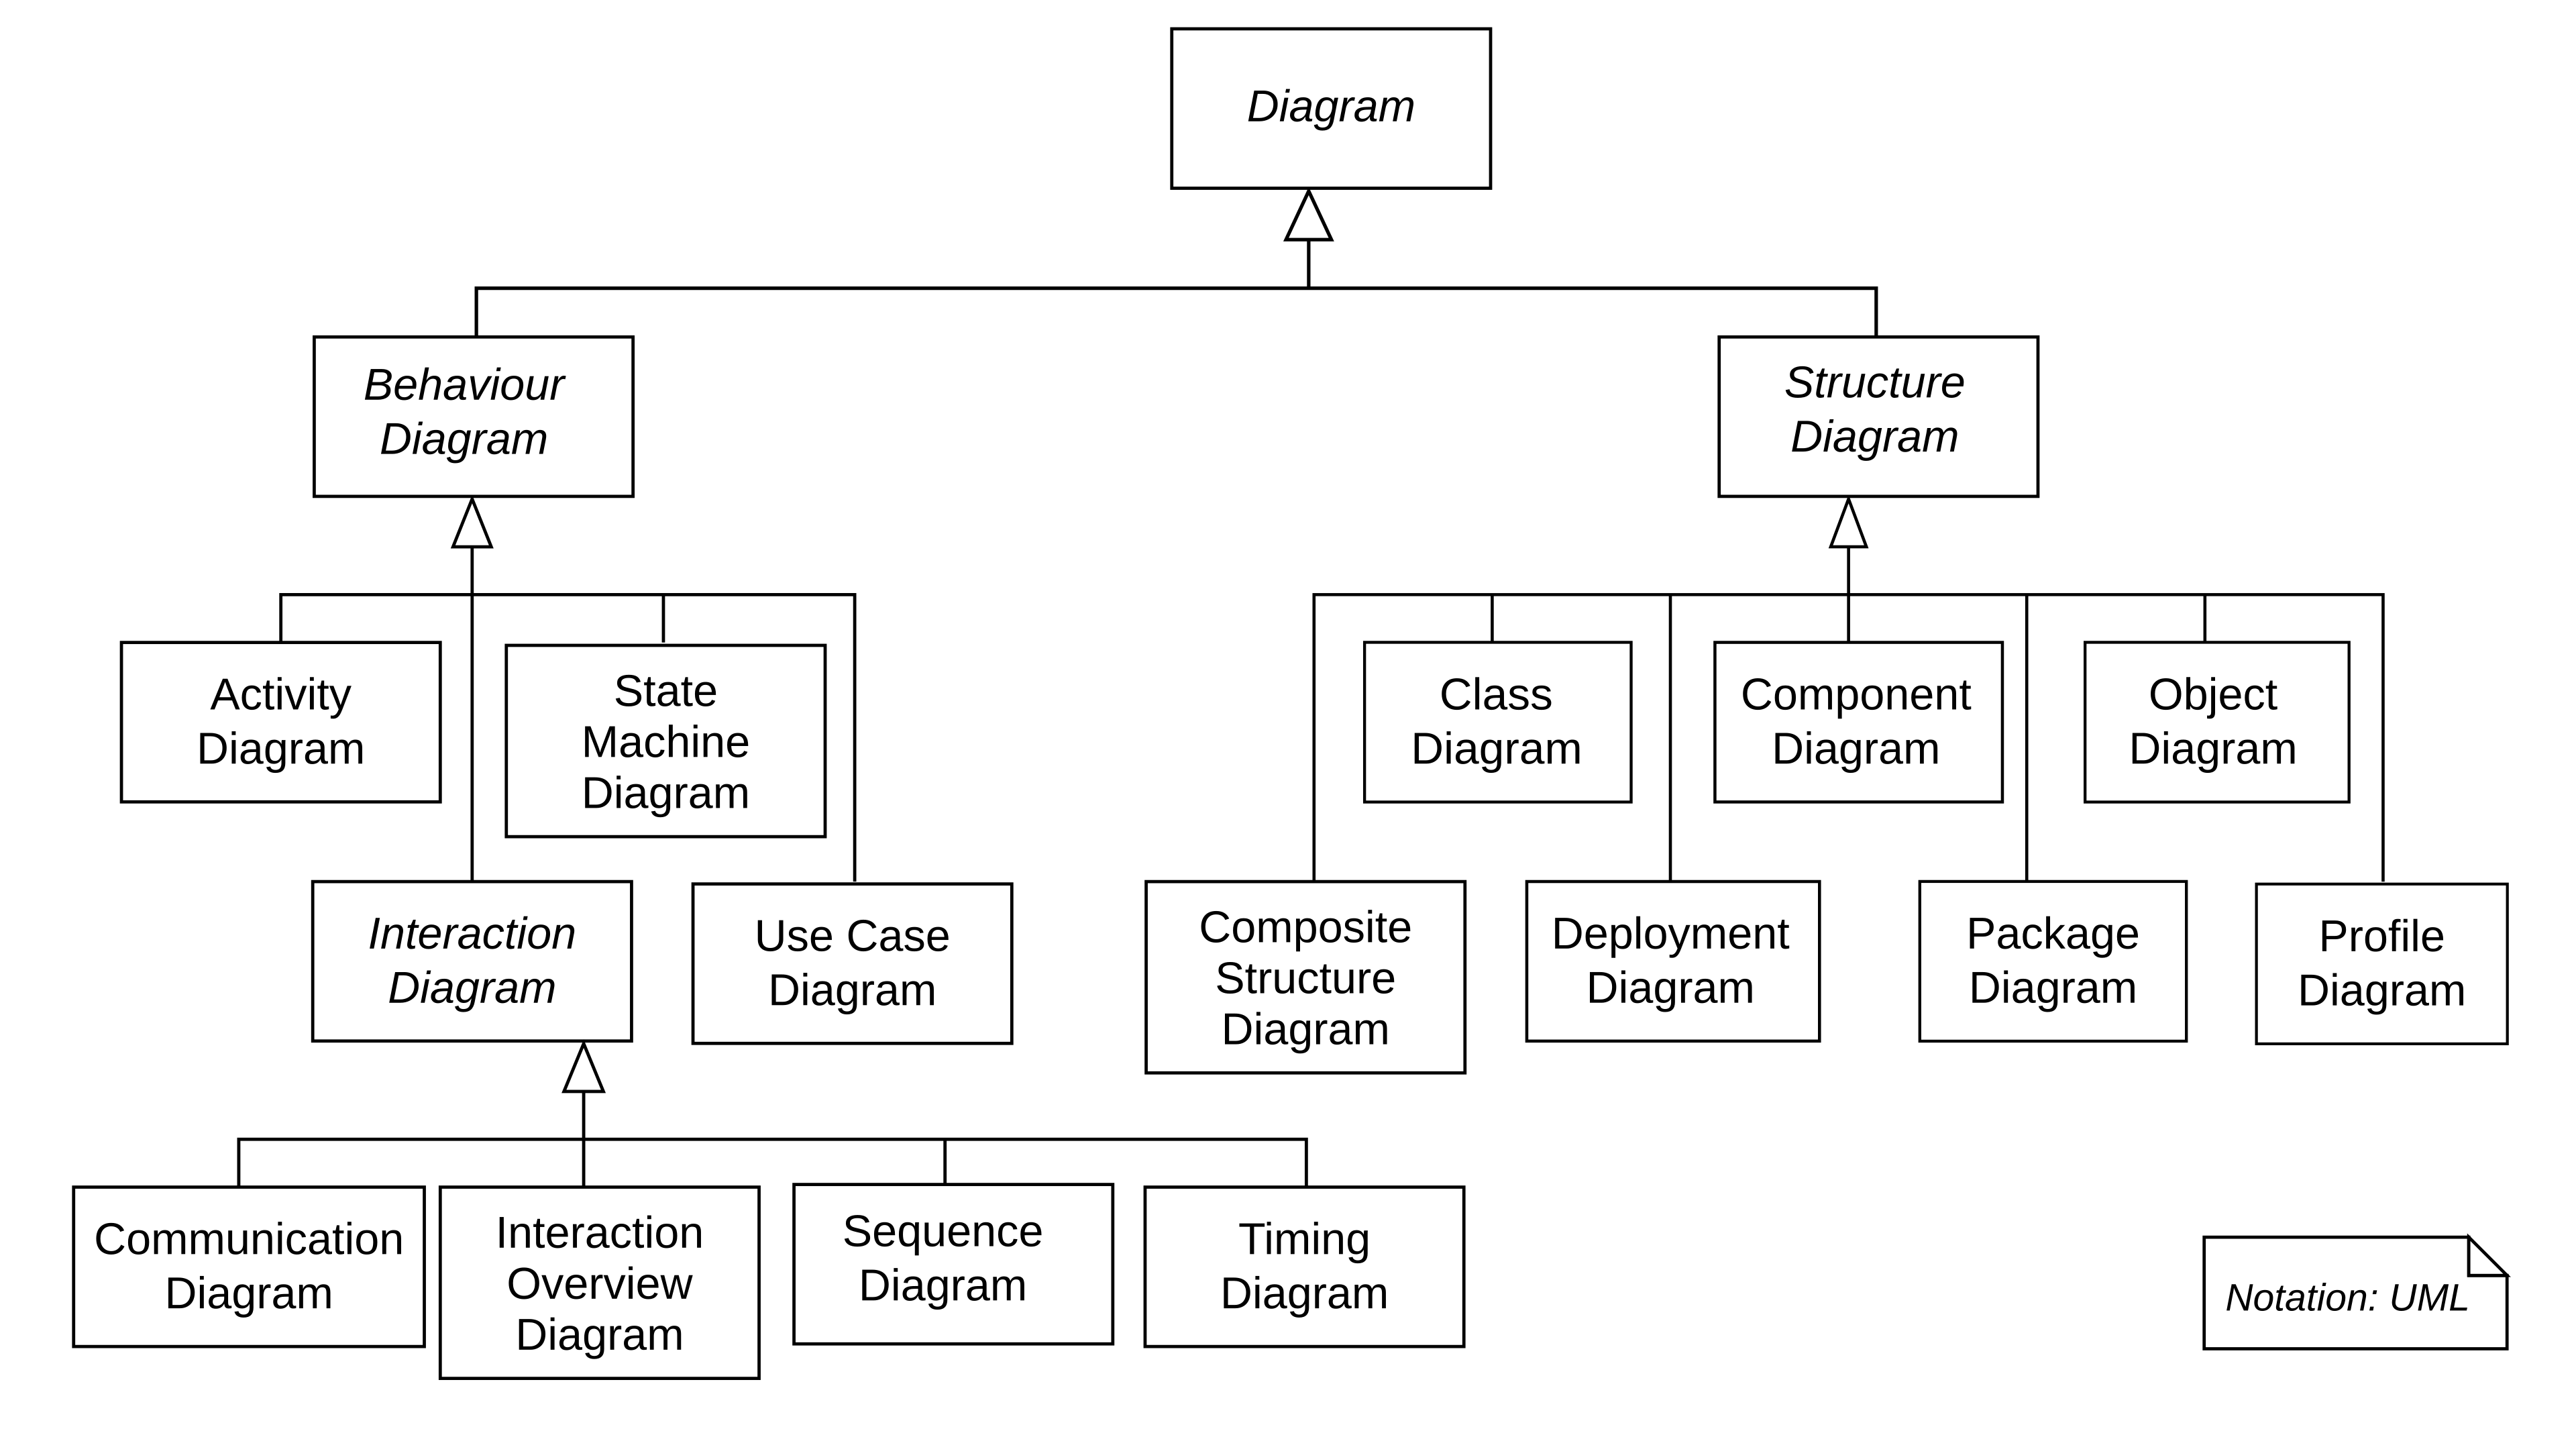
\includegraphics[width=0.9\textwidth]{imgs/UML_diagrams_overview.svg.png}
    \end{center}

\end{frame}

\begin{frame}
    \frametitle{Key UML Diagrams for Software Modelling}
    UML has 14 official diagram types, but not all are equally useful for software system modelling. Some are more relevant for hardware design, business process modelling, or database design.
    
    \vspace{0.3cm}
    \textbf{Top 4 Most Used UML Diagrams:}
    \begin{enumerate}
        \item \textbf{Use Case Diagrams} (Interaction/External)
        \item \textbf{Sequence Diagrams} (Interaction)
        \item \textbf{Class Diagrams} (Structural / OOP)
        \item \textbf{Activity Diagrams} (Behavioral)
    \end{enumerate}
\end{frame}

\begin{frame}[fragile]
    \frametitle{1. Use Case Diagrams}
    Show the interactions between a system and its environment (users or other systems).
    
    \vspace{0.3cm}
    \begin{columns}
        \column{0.5\textwidth}
        \begin{itemize}
            \item \textbf{Actors:} Roles played by human users or external hardware/systems (stick figures).
            \item \textbf{Use Cases:} The goal or action (ovals).
            \item \textbf{System Boundary:} The scope of your software (box).
        \end{itemize}
        
        \column{0.5\textwidth}
        \centering
        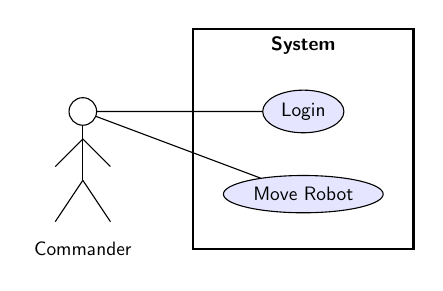
\begin{tikzpicture}[scale=0.7, transform shape]
            % System Boundary
            \draw[thick] (0, 0) rectangle (4, 4);
            \node at (2, 3.7) {\textbf{System}};
            
            % Use Cases
            \node[ellipse, draw, fill=blue!10] (uc1) at (2, 2.5) {Login};
            \node[ellipse, draw, fill=blue!10] (uc2) at (2, 1) {Move Robot};
            
            % Actor
            \node[circle, draw, minimum size=0.5cm] (head) at (-2, 2.5) {};
            \draw (-2, 2.25) -- (-2, 1.25); % body
            \draw (-2, 2.0) -- (-2.5, 1.5); % left arm
            \draw (-2, 2.0) -- (-1.5, 1.5); % right arm
            \draw (-2, 1.25) -- (-2.5, 0.5); % left leg
            \draw (-2, 1.25) -- (-1.5, 0.5); % right leg
            \node at (-2, 0) {Commander};
            
            % Connections
            \draw (head) -- (uc1);
            \draw (head) -- (uc2);
        \end{tikzpicture}
    \end{columns}
\end{frame}

\begin{frame}
    \frametitle{1. Use Case Diagrams}
    \textbf{Example: an online pizza Delivery System}
    \begin{center}
        
    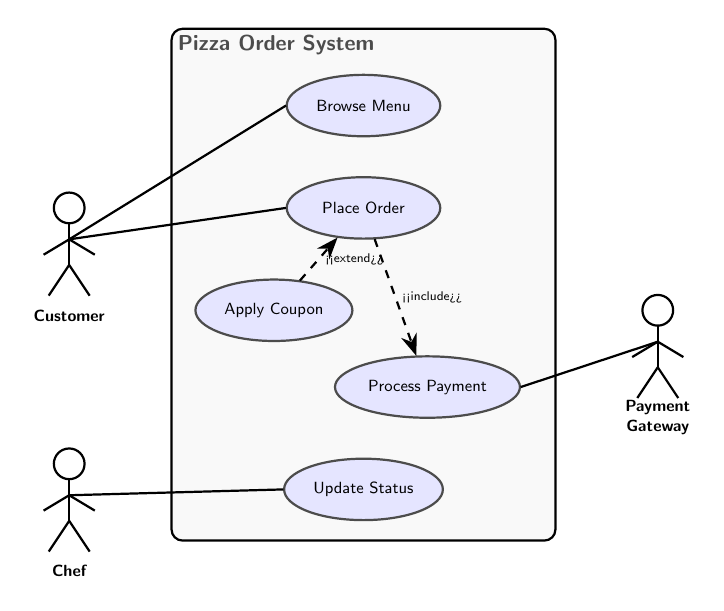
\begin{tikzpicture}[
        scale=0.65, transform shape,
        % Style for Use Cases (Ellipses)
        usecase/.style={
            ellipse, draw=black!70, thick, fill=blue!10,
            minimum width=3cm, minimum height=1.2cm, 
            align=center, font=\small
        },
        % Reusable "pic" for stick-figure Actors
        actor/.pic={
            \node[circle, draw, thick, minimum size=0.6cm, fill=white] (-head) at (0,0) {};
            \draw[thick] (-head.south) -- ++(0,-0.8) coordinate (-pelvis);
            \draw[thick] (-pelvis) -- ++(-0.4,-0.6);
            \draw[thick] (-pelvis) -- ++(0.4,-0.6);
            \draw[thick] ([yshift=-0.3cm]-head.south) coordinate (-chest) -- ++(-0.5,-0.3);
            \draw[thick] (-chest) -- ++(0.5,-0.3);
            \node[align=center, font=\small\bfseries, yshift=-2.1cm] at (0,0) {\tikzpictext};
        }
    ]

        % 1. System Boundary
        \draw[thick, rounded corners, fill=gray!5] (-1, -7.5) rectangle (6.5, 2.5);
        \node[anchor=north west, font=\large\bfseries, text=black!70] at (-1, 2.5) {Pizza Order System};

        % 2. Use Cases
        \node[usecase] (browse) at (2.75, 1) {Browse Menu};
        \node[usecase] (order)  at (2.75, -1) {Place Order};
        \node[usecase] (coupon) at (1, -3) {Apply Coupon};
        \node[usecase] (pay)    at (4, -4.5) {Process Payment};
        \node[usecase] (status) at (2.75, -6.5) {Update Status};

        % 3. Actors
        % We pass the name of the actor via [pic text=...]
        \pic (customer) at (-3, -1)   [pic text=Customer] {actor};
        \pic (chef)     at (-3, -6) [pic text=Chef] {actor};
        \pic (gateway)  at (8.5, -3)  [pic text=Payment\\Gateway] {actor};

        % 4. Associations (Connecting actors to use cases)
        % The (-chest) coordinate was defined inside the \pic to anchor lines cleanly
        \draw[thick] (customer-chest) -- (browse.west);
        \draw[thick] (customer-chest) -- (order.west);
        \draw[thick] (chef-chest)     -- (status.west);
        \draw[thick] (gateway-chest)  -- (pay.east);

        % 5. Relationships (Includes / Extends)
        \draw[-{Stealth[scale=1.2]}, dashed, thick] (order) -- (pay) 
            node[midway, right, font=\scriptsize] {<<include>>};
            
    \draw[-{Stealth[scale=1.2]}, dashed, thick] (coupon) -- (order) 
            node[midway, right, font=\scriptsize] {<<extend>>};

    \end{tikzpicture}

    \end{center}
\end{frame}

\begin{frame}
    \frametitle{2. Sequence Diagrams}

    \begin{itemize}
        \item Sequence diagrams in the UML are primarily used to
model the interactions between the actors and the objects in a system and the interactions between them.
        \item As the name implies, a sequence diagram shows the
\textbf{sequence of interactions during a particular use case} or
use case instance.
        \item The objects and actors involved are listed along the top
of the diagram, with a dotted line drawn vertically from
these.
    \end{itemize}
    
    
    
    % \begin{itemize}
    %     \item \textbf{Lifelines:} Vertical dashed lines representing the lifespan of an object.
    %     \item \textbf{Messages:} Horizontal arrows showing calls, returns, or data transfers.
    %     \item \textbf{Activation Boxes:} Rectangles on the lifeline showing when an object is actively processing.
    %     \item \textbf{Time:} Reads from top to bottom.
    % \end{itemize}
\end{frame}

\begin{frame}[fragile]
    \frametitle{2. Sequence Diagrams: Medical Receptionist}
    Sequence diagrams model the sequence of interactions during a particular use case. 
    
    \vspace{0.2cm}
    \centering
    \resizebox{\textwidth}{!}{
    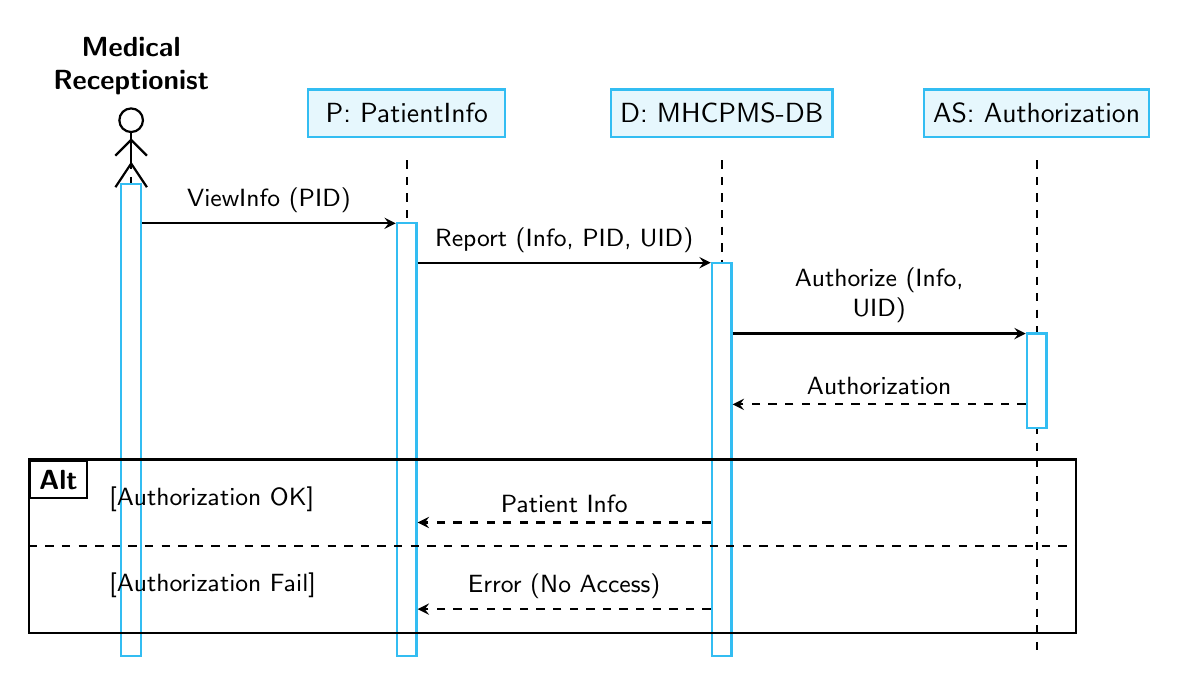
\begin{tikzpicture}[
        actor/.style={draw=none, align=center, font=\bfseries},
        object/.style={rectangle, draw=cyan!80, fill=cyan!10, thick, minimum width=2.5cm, minimum height=0.6cm, align=center},
        lifeline/.style={dashed, thick},
        activity/.style={rectangle, draw=cyan!80, fill=white, thick, minimum width=0.25cm},
        msg/.style={->, >=stealth, thick},
        reply/.style={->, >=stealth, dashed, thick}
    ]
        % Headers
        \node[actor] (rec) at (0,0) {Medical\\Receptionist};
        % Draw stick figure for receptionist
        \draw[thick] (rec.south) ++(0,-0.2) circle (0.15);
        \draw[thick] (rec.south) ++(0,-0.35) -- ++(0,-0.4);
        \draw[thick] (rec.south) ++(0,-0.45) -- ++(-0.2,-0.2);
        \draw[thick] (rec.south) ++(0,-0.45) -- ++(0.2,-0.2);
        \draw[thick] (rec.south) ++(0,-0.75) -- ++(-0.2,-0.3);
        \draw[thick] (rec.south) ++(0,-0.75) -- ++(0.2,-0.3);
        
        \node[object] (p) at (3.5, -0.6) {P: PatientInfo};
        \node[object] (d) at (7.5, -0.6) {D: MHCPMS-DB};
        \node[object] (as) at (11.5, -0.6) {AS: Authorization};

        % Lifelines
        \draw[lifeline] (0,-1.2) -- (0,-7.5);
        \draw[lifeline] (3.5,-1.2) -- (3.5,-7.5);
        \draw[lifeline] (7.5,-1.2) -- (7.5,-7.5);
        \draw[lifeline] (11.5,-1.2) -- (11.5,-7.5);

        % Activity Boxes
        \node[activity, minimum height=6cm] (act_rec) at (0,-4.5) {};
        \node[activity, minimum height=5.5cm] (act_p) at (3.5,-4.75) {};
        \node[activity, minimum height=5cm] (act_d) at (7.5,-5.0) {};
        \node[activity, minimum height=1.2cm] (act_as) at (11.5,-4) {};

        % Messages
        \draw[msg] (act_rec.east |- 0,-2) -- (act_p.west |- 0,-2) node[midway, above, font=\small] {ViewInfo (PID)};
        \draw[msg] (act_p.east |- 0,-2.5) -- (act_d.west |- 0,-2.5) node[midway, above, font=\small] {Report (Info, PID, UID)};
        \draw[msg] (act_d.east |- 0,-3.4) -- (act_as.west |- 0,-3.4) node[midway, above, align=center, font=\small] {Authorize (Info,\\UID)};
        \draw[reply] (act_as.west |- 0,-4.3) -- (act_d.east |- 0,-4.3) node[midway, above, font=\small] {Authorization};

        % Alt Box
        \draw[draw=black, thick] (-1.3, -5) rectangle (12, -7.2);
        \node[draw=black, fill=white, thick, anchor=north west] at (-1.3, -5) {\textbf{Alt}};
        \draw[dashed, thick] (-1.3, -6.1) -- (12, -6.1);

        % Alt Conditions & Returns
        \node[anchor=west, font=\small] at (-0.4, -5.5) {[Authorization OK]};
        \draw[reply] (act_d.west |- 0,-5.8) -- (act_p.east |- 0,-5.8) node[midway, above, font=\small] {Patient Info};

        \node[anchor=west, font=\small] at (-0.4, -6.6) {[Authorization Fail]};
        \draw[reply] (act_d.west |- 0,-6.9) -- (act_p.east |- 0,-6.9) node[midway, above, font=\small] {Error (No Access)};
    \end{tikzpicture}
    }
\end{frame}

\begin{frame}
    \frametitle{2. Sequence Diagram Components}
    \small
    How do we read the Medical Receptionist model? You read the sequence of interactions from top to bottom.
    
    \vspace{0.3cm}
    \begin{itemize}
        \item \textbf{Actors \& Objects:} Listed along the top. A dotted vertical line drops down from each, representing the object's \textit{lifeline}.
        \item \textbf{Activation Boxes (Rectangles):} Placed on the lifeline to indicate the time the object instance is actively involved in the computation.
        \item \textbf{Messages (Annotated Arrows):} Indicate calls to objects. The annotations show parameters (e.g., \texttt{PID}) and return values.
        \item \textbf{Alternatives (Alt Box):} Used to denote conditional logic. The box is divided into sections with conditions in square brackets (e.g., \texttt{[Authorization OK]}).
    \end{itemize}
    \vspace{0.2cm}
    \textit{Note: You don't have to include every single interaction; focus on the critical logic!}
\end{frame}

%------------------------------------------------------------
% CLASS DIAGRAMS
%------------------------------------------------------------

\begin{frame}
    \frametitle{3. Class Diagrams \& Object-Oriented Programming}
    Class diagrams are the backbone of Object-Oriented Programming (OOP). They show the object classes in the system and their associations.
    
    \vspace{0.3cm}
    \textbf{Mapping OOP to UML:}
    \begin{itemize}
        \item \textbf{Encapsulation:} A class groups Data (Attributes) and Behavior (Methods/Operations) together.
        \item \textbf{Inheritance:} "Is-a" relationship (e.g., a \texttt{Drone} is a type of \texttt{Robot}). Shown with a hollow arrow.
        \item \textbf{Association:} "Has-a" or "Uses-a" relationship (e.g., a \texttt{Commander} controls a \texttt{Robot}).
    \end{itemize}
\end{frame}


\begin{frame}[fragile]
    \frametitle{3. Class Diagrams: Attributes \& Operations}
    Class diagrams describe the types of objects within the system and their relationships.
    
    \vspace{0.2cm}
    \begin{columns}
        \column{0.60\textwidth}
        \begin{itemize}
            \item Rectangles are divided into three parts: class name, attributes, and operations (methods).
            \item \textbf{Attributes} characterize the class and define the state of objects within the class.
            \item \textbf{Visibility Modifiers:}
                \begin{itemize}
                \item \texttt{+} Public (Accessible anywhere)
                \item \texttt{-} Private (Encapsulated/Hidden)
                \item \texttt{\#} Protected (Accessible to subclasses)
                \end{itemize}
        \end{itemize}
        
        \column{0.40\textwidth}
        \centering
        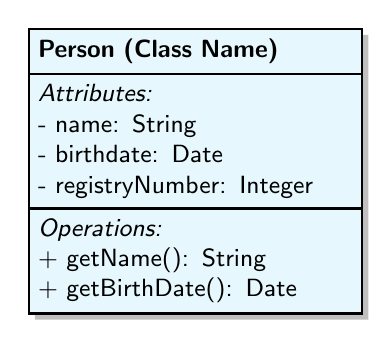
\begin{tikzpicture}[
            classbox/.style={
                rectangle split, rectangle split parts=3, 
                draw=black, fill=white, thick, 
                text width=4cm, align=left, 
                font=\small, drop shadow
            }
        ]
            \node[classbox, fill=cyan!10] (person) {
                \nodepart{one} \centering \textbf{Person (Class Name)}
                \nodepart{two} 
                \textit{Attributes:}\\
                - name: String\\
                - birthdate: Date\\
                - registryNumber: Integer
                \nodepart{three}
                \textit{Operations:}\\
                + getName(): String\\
                + getBirthDate(): Date
            };
        %     \node[align=left, font=\footnotesize, right=1cm of robot] {
        %     \textbf{Visibility Modifiers:}\\
        %     \texttt{+} Public (Accessible anywhere)\\
        %     \texttt{-} Private (Encapsulated/Hidden)\\
        %     \texttt{\#} Protected (Accessible to subclasses)
        % };
        \end{tikzpicture}
    \end{columns}
\end{frame}

\begin{frame}[fragile]
    \frametitle{3. Class Diagrams: Associations \& Multiplicity}
    \begin{itemize}
        \item \textbf{Associations:} Relationships between two classes are shown as lines connecting them, often with a label to describe the relationship.
        \item \textbf{Multiplicity:} The cardinality of the relationship (how many instances of a class can be associated with another) is represented at the ends of an association line.
    \end{itemize}
    
    \vspace{0.4cm}
    \centering
    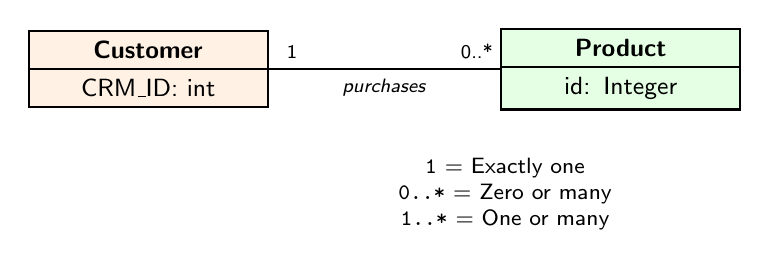
\begin{tikzpicture}[
        classbox/.style={
            rectangle split, rectangle split parts=2, 
            draw=black, fill=white, thick, 
            text width=2.8cm, align=center, 
            font=\small
        }
    ]
        \node[classbox, fill=orange!10] (cust) at (0,0) {
            \textbf{Customer}
            \nodepart{two} CRM\_ID: int
        };
        
        \node[classbox, fill=green!10] (prod) at (6,0) {
            \textbf{Product}
            \nodepart{two} id: Integer
        };
        
        \draw[thick] (cust.east) -- (prod.west) 
            node[pos=0.1, above, font=\scriptsize] {1}
            node[pos=0.9, above, font=\scriptsize] {0..*}
            node[midway, below, font=\scriptsize] {\textit{purchases}};
            
        \node[align=center, font=\footnotesize, below=1cm of cust.east, xshift=3cm] {
            \texttt{1} = Exactly one \\
            \texttt{0..*} = Zero or many \\
            \texttt{1..*} = One or many
        };
    \end{tikzpicture}
\end{frame}

\begin{frame}[fragile]
    \frametitle{3. Class Diagrams: Aggregation vs Composition}
    \begin{itemize}
        \item \textbf{Aggregation:} A "whole-part" relationship where the component part can exist independently. Represented as a hollow diamond at the aggregate (whole) end.
        \item \textbf{Composition:} A stronger form indicating the part cannot exist without the whole. Depicted as a filled diamond at the whole end.
    \end{itemize}
    
    \vspace{0.2cm}
    \centering
    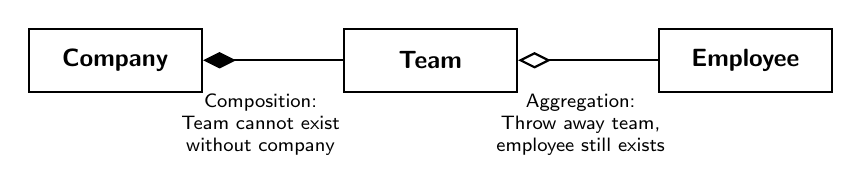
\begin{tikzpicture}[
        classbox/.style={draw=black, fill=white, thick, minimum width=2.2cm, minimum height=0.8cm, align=center, font=\small},
        comp/.style={-{Diamond[scale=1.5]}, thick},
        agg/.style={-{Diamond[open, scale=1.5]}, thick}
    ]
        \node[classbox] (team) at (0,0) {\textbf{Team}};
        \node[classbox] (company) at (-4,0) {\textbf{Company}};
        \node[classbox] (emp) at (4,0) {\textbf{Employee}};

        % Diamonds point to the "Whole"
        \draw[comp] (team.west) -- (company.east);
        \draw[agg] (emp.west) -- (team.east);
        
        \node[align=center, font=\scriptsize, below right=0.3cm and -0.4cm of company.east] {Composition:\\Team cannot exist\\without company};
        \node[align=center, font=\scriptsize, below right=0.3cm and -0.4cm of team.east] {Aggregation:\\Throw away team,\\employee still exists};
    \end{tikzpicture}
\end{frame}

\begin{frame}[fragile]
    \frametitle{3. Class Diagrams: Inheritance (Generalization)}
    \begin{itemize}
        \item \textbf{Inheritance:} Represents a relationship where one class (the subclass) is based on another class (the superclass), inheriting its features.
        \item Depicted as a line with a \textbf{hollow triangle} pointing towards the superclass.
    \end{itemize}
    
    \vspace{0.2cm}
    \begin{center}
        
    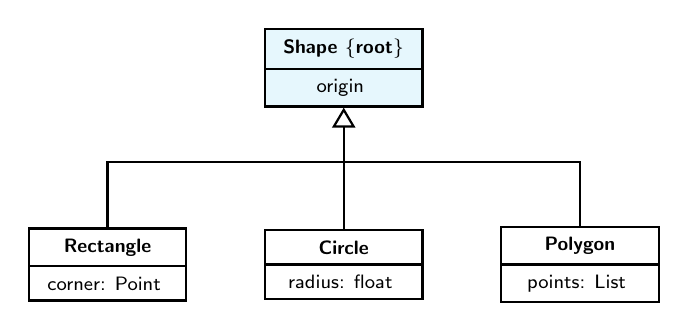
\begin{tikzpicture}[
        classbox/.style={rectangle split, rectangle split parts=2, draw=black, fill=white, thick, minimum width=2cm, align=center, font=\scriptsize},
        inherit/.style={-{Triangle[open, scale=1.5]}, thick}
    ]
        \node[classbox, fill=cyan!10] (shape) at (0,0) {
            \textbf{Shape \{root\}}
            \nodepart{two} origin
        };
        \node[classbox] (rect) at (-3,-2.5) {
            \textbf{Rectangle}
            \nodepart{two} corner: Point
        };
        \node[classbox] (circle) at (0,-2.5) {
            \textbf{Circle}
            \nodepart{two} radius: float
        };
        \node[classbox] (poly) at (3,-2.5) {
            \textbf{Polygon}
            \nodepart{two} points: List
        };

        \draw[thick] (rect.north) |- (0,-1.2);
        \draw[thick] (poly.north) |- (0,-1.2);
        \draw[inherit] (0,-1.2) -- (shape.south);
        \draw[thick] (circle.north) -- (0,-1.2);
    \end{tikzpicture}
    \end{center}
\end{frame}

%------------------------------------------------------------
% ACTIVITY DIAGRAMS
%------------------------------------------------------------

\begin{frame}
    \frametitle{4. Activity Diagrams}
    Activity diagrams show the sequence of activities involved in a process or data processing. They are similar to flowcharts.
    
    
    
    \begin{itemize}
        \item Good for mapping out complex business logic.
        \item Uses \textbf{Decision Nodes} (diamonds) for branching logic (e.g., ``Is Battery $>$ 10\%?'').
        \item Uses \textbf{Forks} and \textbf{Joins} (thick black bars) to show concurrent, parallel processing.
    \end{itemize}
\end{frame}

\begin{frame}[fragile]
    \frametitle{4. Activity Diagrams: Basics}
    Activity diagrams show the sequence of activities involved in a process or data processing.
    
    \vspace{0.3cm}
    \begin{itemize}
        \item \textbf{Start/End:} The start of a process is indicated by a filled circle; the end by a filled circle inside another circle.
        \item \textbf{Activities:} Rectangles with round corners represent the specific sub-processes that must be carried out.
        \item \textbf{Flow:} Arrows represent the flow of work from one activity to another.
    \end{itemize}
    
    \vspace{0.2cm}
    \centering
    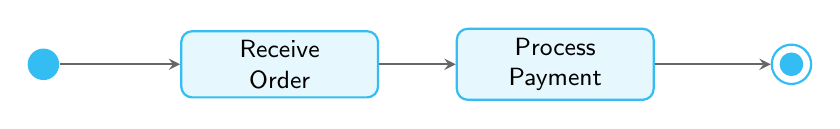
\begin{tikzpicture}[
        start/.style={circle, fill=cyan!80, minimum size=0.4cm},
        end/.style={circle, draw=cyan!80, thick, inner sep=0pt, minimum size=0.5cm, path picture={\fill[cyan!80] (path picture bounding box.center) circle (0.15cm);}},
        activity/.style={rectangle, draw=cyan!80, fill=cyan!10, thick, rounded corners, minimum width=2.5cm, minimum height=0.8cm, align=center, font=\small},
        arrow/.style={->, >=stealth, thick, gray!80!black}
    ]
        \node[start] (start) at (0, 0) {};
        \node[activity] (act1) at (3, 0) {Receive\\Order};
        \node[activity] (act2) at (6.5, 0) {Process\\Payment};
        \node[end] (end) at (9.5, 0) {};

        \draw[arrow] (start) -- (act1);
        \draw[arrow] (act1) -- (act2);
        \draw[arrow] (act2) -- (end);
    \end{tikzpicture}
\end{frame}

\begin{frame}[fragile]
    \frametitle{4. Activity Diagrams: Coordination \& Decisions}
    
    \begin{itemize}
        \item \textbf{Coordination (Forks/Joins):} A solid bar indicates activity coordination. When flows lead to a solid bar, all of these activities must be complete before progress is possible.
        \item \textbf{Decisions (Guards):} Arrows may be annotated with guards (in square brackets) that indicate the condition when that flow is taken (e.g., \texttt{[Dangerous]}).
    \end{itemize}
    
    \vspace{0.2cm}
    \centering
    \resizebox{0.9\textwidth}{!}{%
    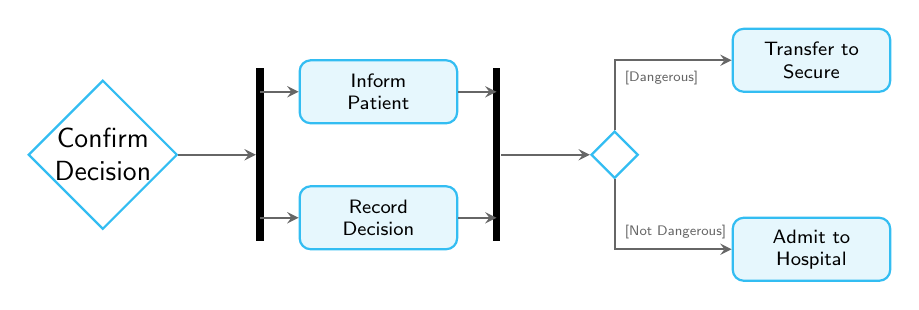
\begin{tikzpicture}[%
        activity/.style={rectangle, draw=cyan!80, fill=cyan!10, thick, rounded corners, minimum width=2cm, minimum height=0.8cm, align=center, font=\scriptsize},
        decision/.style={diamond, draw=cyan!80, thick, minimum size=0.6cm, inner sep=0pt, align=center},
        bar/.style={rectangle, fill=black, minimum width=0.1cm, minimum height=2.2cm, inner sep=0pt},
        arrow/.style={->, >=stealth, thick, gray!80!black}%
    ]
        \node[decision, fill=white] (start) at (0, 0) {Confirm\\Decision};
        \node[bar] (fork) at (2, 0) {};
        
        \node[activity] (inf) at (3.5, 0.8) {Inform\\Patient};
        \node[activity] (rec) at (3.5, -0.8) {Record\\Decision};
        
        \node[bar] (join) at (5, 0) {};
        \node[decision, fill=white] (dec) at (6.5, 0) {};
        
        \node[activity] (sec) at (9, 1.2) {Transfer to\\Secure};
        \node[activity] (adm) at (9, -1.2) {Admit to\\Hospital};

        \draw[arrow] (start) -- (fork);
        \draw[arrow] (fork.north |- inf.west) -- (inf.west);
        \draw[arrow] (fork.south |- rec.west) -- (rec.west);
        
        \draw[arrow] (inf.east) -- (join.north |- inf.east);
        \draw[arrow] (rec.east) -- (join.south |- rec.east);
        
        \draw[arrow] (join) -- (dec);
        \draw[arrow] (dec) |- node[near start, above right, font=\tiny] {[Dangerous]} (sec.west);
        \draw[arrow] (dec) |- node[near start, below right, font=\tiny] {[Not Dangerous]} (adm.west);
    \end{tikzpicture}%
    }%
\end{frame}

% \begin{frame}
%     \frametitle{3. Class Diagrams \& Object-Oriented Programming}
%     Class diagrams are the backbone of Object-Oriented Programming (OOP). They show the object classes in the system and their associations.
    
%     \vspace{0.3cm}
%     \textbf{Mapping OOP to UML:}
%     \begin{itemize}
%         \item \textbf{Encapsulation:} A class groups Data (Attributes) and Behavior (Methods/Operations) together.
%         \item \textbf{Inheritance:} "Is-a" relationship (e.g., a \texttt{Drone} is a type of \texttt{Robot}). Shown with a hollow arrow.
%         \item \textbf{Association:} "Has-a" or "Uses-a" relationship (e.g., a \texttt{Commander} controls a \texttt{Robot}).
%     \end{itemize}
% \end{frame}


% \begin{frame}[fragile]
%     \frametitle{Structure of a Class Node}
%     \centering
%     \begin{tikzpicture}[
%         classbox/.style={
%             rectangle split, rectangle split parts=3, 
%             draw=black, fill=white, thick, 
%             text width=4cm, align=left, 
%             font=\small, drop shadow
%         }
%     ]
%         \node[classbox, fill=cyan!10] (robot) {
%             \nodepart{one} \centering \textbf{Robot (Class Name)}
%             \nodepart{two} 
%             - robotID: String\\
%             - batteryLevel: int\\
%             - positionX: int\\
%             - positionY: int
%             \nodepart{three}
%             + getStatus(): JSON\\
%             + move(x: int, y: int): bool\\
%             - calculatePath(): void
%         };
        
%         \node[align=left, font=\footnotesize, right=1cm of robot] {
%             \textbf{Visibility Modifiers:}\\
%             \texttt{+} Public (Accessible anywhere)\\
%             \texttt{-} Private (Encapsulated/Hidden)\\
%             \texttt{\#} Protected (Accessible to subclasses)
%         };
%     \end{tikzpicture}
% \end{frame}

% \begin{frame}
%     \frametitle{4. Activity Diagrams}
%     Activity diagrams show the sequence of activities involved in a process or data processing. They are similar to flowcharts.
    
    
    
%     \begin{itemize}
%         \item Good for mapping out complex business logic.
%         \item Uses \textbf{Decision Nodes} (diamonds) for branching logic (e.g., ``Is Battery $>$ 10\%?'').
%         \item Uses \textbf{Forks} and \textbf{Joins} (thick black bars) to show concurrent, parallel processing.
%     \end{itemize}
% \end{frame}


%------------------------------------------------------------
% SUMMARY OF DIAGRAMS
%------------------------------------------------------------

\begin{frame}
    \frametitle{Summary of UML Diagrams}
    We have explored four key UML diagrams, each providing a unique perspective on the software system:
    
    \vspace{0.3cm}
    \begin{itemize}
        \item \textbf{Use Case Diagrams (External Perspective):} Model the context of the system and its interactions with outside actors.
        \item \textbf{Sequence Diagrams (Interaction Perspective):} Detail how objects interact over time to complete a specific use case.
        \item \textbf{Class Diagrams (Structural Perspective):} Define the static structure, showing classes, attributes, operations, and relationships.
        \item \textbf{Activity Diagrams (Behavioral Perspective):} Illustrate the dynamic flow of control or data from activity to activity.
    \end{itemize}
    
    \vspace{0.3cm}
    \textit{No single diagram captures everything. A complete system model requires multiple views!}
\end{frame}

\begin{frame}
    \frametitle{When to Use Which Diagram?}
    \centering
    \rowcolors{1}{cyan!10}{white}
    \resizebox{\textwidth}{!}{
    \begin{tabular}{|p{3cm}|p{3cm}|p{5cm}|p{3.5cm}|}
        \hline
        \rowcolor{cyan!80}
        \textbf{Diagram} & \textbf{Focus} & \textbf{When to Use?} & \textbf{Key Elements} \\
        \hline
        \textbf{Use Case} & External / Context & To capture system requirements and show what the system does for its users. & Actors, Use Cases, Boundaries \\
        \textbf{Sequence} & Interaction / Time & To design the step-by-step message flow between objects for a specific scenario. & Lifelines, Messages, Activation Boxes \\
        \textbf{Class} & Structural / OOP & To design the static architecture, database schema, or object-oriented code structure. & Classes, Attributes, Methods, Associations \\
        \textbf{Activity} & Behavioral / Flow & To model complex business logic, parallel processes, or algorithms. & Activities, Decisions, Forks, Joins \\
        \hline
    \end{tabular}
    }
\end{frame}

%------------------------------------------------------------
\section{Interactive Hands-On: Let's Model!}
%------------------------------------------------------------

\begin{frame}
    \frametitle{Interactive Exercise: The Scenario}
    \begin{block}{Scenario: "PizzaOps" Online Delivery System}
        We are building a software system for a local pizza shop. 
        \begin{itemize}
            \item \textbf{Customers} can log in, browse the menu, and place an order.
            \item \textbf{Chefs} receive the order in the kitchen and update its status to "Baking".
            \item Payments are processed securely via a \textbf{Third-Party Payment Gateway} (like Stripe).
        \end{itemize}
    \end{block}
    
    \vspace{0.5cm}
    \textit{Question to the room: If we want to map out WHO uses this system and WHAT they can do, which diagram do we start with?}
\end{frame}

\begin{frame}
    \frametitle{Step 1: The Use Case Diagram}
    \textbf{Task:} Identify the Actors and Use Cases.
    
    \vspace{0.5cm}
    \textit{Question to the room: Who are the actors and what are the use cases?}
\end{frame}

\begin{frame}
    \frametitle{Step 1: The Use Case Diagram (Solution)}
    \textbf{Actors:}
    \begin{itemize}
        \item Customer (Human)
        \item Chef (Human)
        \item Payment Gateway (External System)
    \end{itemize}
    
    \vspace{0.2cm}
    \textbf{Use Cases (What are the bubbles?):}
    \begin{itemize}
        \item Browse Menu
        \item Place Order
        \item Process Payment
        \item Update Order Status
    \end{itemize}
\end{frame}

\begin{frame}
    \frametitle{Step 2: The Sequence Diagram}
    \textbf{Task:} Let's trace the dynamic timeline of "Placing an Order".
    
    \vspace{0.3cm}
    \textit{Question to the room: What are the "Lifelines" (vertical lines) going to be across the top?}
\end{frame}

\begin{frame}
    \frametitle{Step 2: The Sequence Diagram (Solution)}
    \textbf{Timeline Draft:}
    \begin{enumerate}
        \item \texttt{Customer} sends `submitOrder()` to \texttt{WebInterface}.
        \item \texttt{WebInterface} sends `processCharge()` to \texttt{PaymentGateway}.
        \item \texttt{PaymentGateway} returns `Payment Success`.
        \item \texttt{WebInterface} sends `createTicket()` to \texttt{KitchenSystem}.
    \end{enumerate}
\end{frame}

\begin{frame}[fragile]
    \frametitle{Step 3: The Class Diagram (OOP)}
    \textbf{Task:} Identify the structural Classes, Attributes, and Methods.
    
    \vspace{0.3cm}
    \textit{Question to the room: What are the main classes and their relationships?}
\end{frame}

\begin{frame}[fragile]
    \frametitle{Step 3: The Class Diagram (OOP) (Solution)}
    \centering
    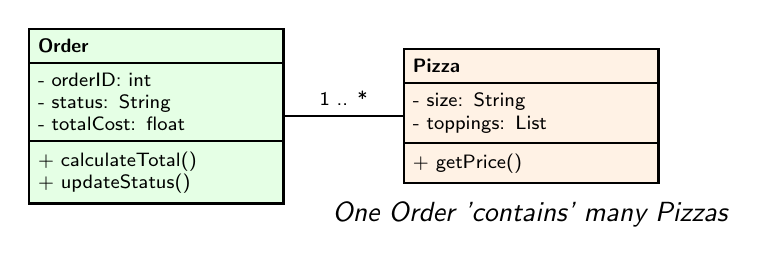
\begin{tikzpicture}[
        classbox/.style={
            rectangle split, rectangle split parts=3, 
            draw=black, fill=white, thick, 
            text width=3cm, align=left, 
            font=\scriptsize
        },
        arrow/.style={->, >=stealth, thick}
    ]
        \node[classbox, fill=green!10] (order) {
            \nodepart{one} \centering \textbf{Order}
            \nodepart{two} 
            - orderID: int\\
            - status: String\\
            - totalCost: float
            \nodepart{three}
            + calculateTotal()\\
            + updateStatus()
        };
        
        \node[classbox, fill=orange!10, right=1.5cm of order] (pizza) {
            \nodepart{one} \centering \textbf{Pizza}
            \nodepart{two} 
            - size: String\\
            - toppings: List
            \nodepart{three}
            + getPrice()
        };
        
        \draw[thick] (order.east) -- (pizza.west) node[midway, above] {\scriptsize 1 .. *};
        \node[below=0.1cm of pizza] {\textit{One Order 'contains' many Pizzas}};
    \end{tikzpicture}
\end{frame}

\begin{frame}[fragile]
    \frametitle{Step 4: The Activity Diagram}
    \textbf{Task:} Map out the business logic for "Processing an Order".
    
    \vspace{0.3cm}
    \textit{Question to the room: What happens if the payment fails?}
\end{frame}

\begin{frame}[fragile]
    \frametitle{Step 4: The Activity Diagram (Solution)}
    \centering
    \resizebox{0.9\textwidth}{!}{%
    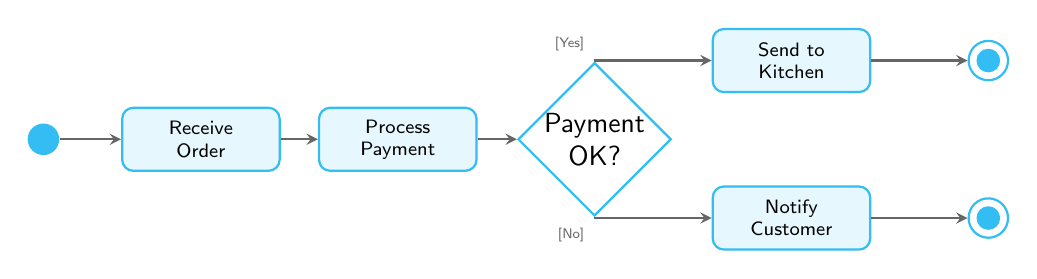
\begin{tikzpicture}[%
        activity/.style={rectangle, draw=cyan!80, fill=cyan!10, thick, rounded corners, minimum width=2cm, minimum height=0.8cm, align=center, font=\scriptsize},
        decision/.style={diamond, draw=cyan!80, thick, minimum size=0.6cm, inner sep=0pt, align=center},
        start/.style={circle, fill=cyan!80, minimum size=0.4cm},
        end/.style={circle, draw=cyan!80, thick, inner sep=0pt, minimum size=0.5cm, path picture={\fill[cyan!80] (path picture bounding box.center) circle (0.15cm);}},
        arrow/.style={->, >=stealth, thick, gray!80!black}%
    ]
        \node[start] (start) at (0, 0) {};
        \node[activity] (recv) at (2, 0) {Receive\\Order};
        \node[activity] (pay) at (4.5, 0) {Process\\Payment};
        \node[decision, fill=white] (dec) at (7, 0) {Payment\\OK?};
        
        \node[activity] (kitchen) at (9.5, 1) {Send to\\Kitchen};
        \node[activity] (fail) at (9.5, -1) {Notify\\Customer};
        
        \node[end] (end1) at (12, 1) {};
        \node[end] (end2) at (12, -1) {};

        \draw[arrow] (start) -- (recv);
        \draw[arrow] (recv) -- (pay);
        \draw[arrow] (pay) -- (dec);
        
        \draw[arrow] (dec) |- node[near start, above left, font=\tiny] {[Yes]} (kitchen.west);
        \draw[arrow] (dec) |- node[near start, below left, font=\tiny] {[No]} (fail.west);
        
        \draw[arrow] (kitchen) -- (end1);
        \draw[arrow] (fail) -- (end2);
    \end{tikzpicture}%
    }%
\end{frame}

%------------------------------------------------------------
\section{Next Steps}
%------------------------------------------------------------

% \begin{frame}
%     \frametitle{This Week's Lab: Modelling Your Robot}
%     In the workshop, you will apply these tools to your Assessment 1 project (The Robot Management System).
    
%     \begin{itemize}
%         \item \textbf{Task 1:} Draw a \textbf{Use Case Diagram} identifying your Commander, Viewer, and Auditor roles.
%         \item \textbf{Task 2:} Draw a \textbf{Class Diagram} for your Python/Node.js backend (e.g., mapping out the Robot API connection).
%         \item \textbf{Task 3:} Draw a \textbf{Sequence Diagram} showing exactly how a "Move" command travels from the UI, through the backend, to the Docker API.
%         \item \textbf{Tooling:} We recommend using \href{https://app.diagrams.net/}{Draw.io}, Lucidchart, or Mermaid.js.
%     \end{itemize}
% \end{frame}

\begin{frame}
    \frametitle{Reading \& Resources}
    \begin{itemize}
        \item \textbf{Recommended Reading:} 
        Sommerville, \textit{Software Engineering 9th Edition}, Chapter 5 (System Modeling).
        % \item \textbf{Mermaid.js:} Highly recommended! It allows you to generate UML diagrams using markdown text directly in your GitHub README files.
        \item \textbf{Next Week:} We will cover \textbf{Software Patterns and Reuse}.
    \end{itemize}
\end{frame}

\begin{frame}
    \frametitle{Q \& A}
    \begin{center}
        \Huge Any Questions?\\\vspace{0.5cm} 
        \normalsize fdelduchetto@lincoln.ac.uk
    \end{center}
\end{frame}

\end{document}